\section{Fast-Opening Valve Design} \label{s:design}
% talk about design requirements
% discuss the initial piston valve design -- what was it, how well did it work, why did it not work


To meet the requirements outlined above, a piston actuated valve was designed, built, and tested at OSU.
The valve utilizes the helium from the high pressure driver tank in HENRI as its working fluid, which decreases the chances of contamination compared to using another working fluid, as well as keeping the required external attachments to a minimum to improve the modularity of the HENRI cartridge.
The piston can fit inside the driver tank and attaches to the driver tank's flange.
The flange is machined to accept a machined plug that attaches to the piston to create a tight seal.
The valve can open rapidly by using the pressure of the helium in the driver tank and fully pulls away from the flange to provide obstruction-free flow into the test section.
\Cref{fig:cad gen 1} shows CAD models of the piston valve, both a concept model and an as-built model.
\Cref{fig:cad concept} shows the concept of the valve and how it attaches to the driver tank flange to sit inside the HENRI cartridge and \Cref{fig:cad lip} shows the as-built piston mount and flange.
The sealing surface has a lip machined into it that helps the metal plug to seal against the surface of the flange.

% obviously put a drawing and/or picture here of the og design -- also include a picture of the whole HENRI assembly with labels, so this all makes sense
\begin{figure}[b!]
    \vspace{16pt}
    \centering
    \begin{subfigure}[t]{0.6\textwidth}
        \centering
        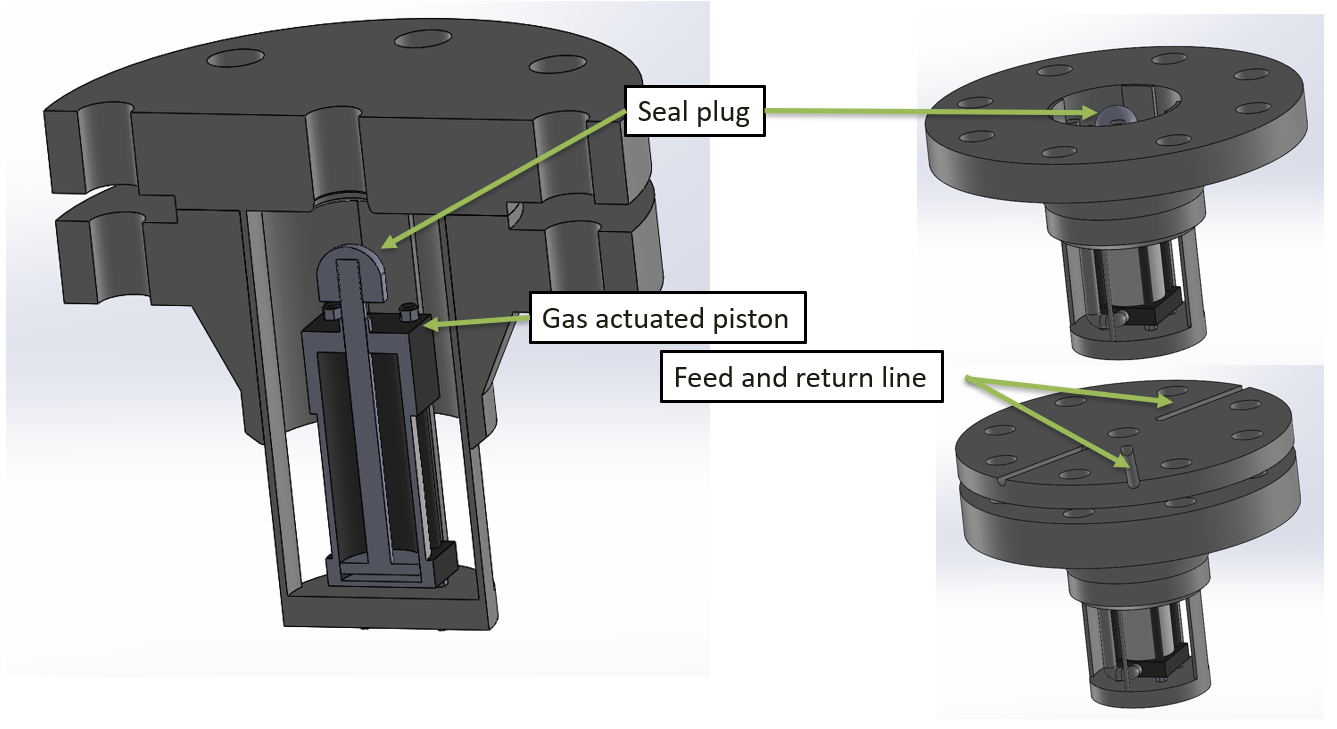
\includegraphics[width=0.8\textwidth]{design/photos/PistonValve_Gen1_CAD_labels.PNG}
        \caption{CAD model of a piston valve concept attached to driver tank flange.}
        \label{fig:cad concept}
    \end{subfigure}
    \hfill
    \begin{subfigure}[t]{0.35\textwidth}
        \centering
        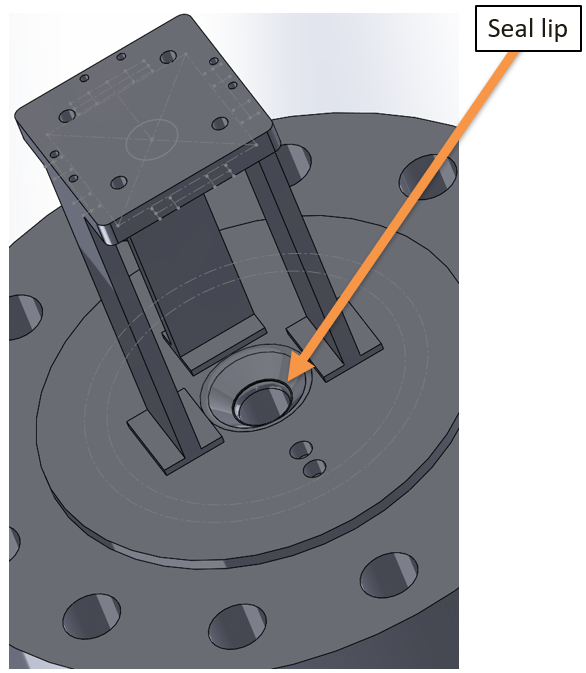
\includegraphics[width=0.8\textwidth]{design/photos/PistonMount_CAD_lip.PNG}
        \caption{As-built CAD model of first piston valve mount and driver tank flange, with sealing lip highlighted.}
        \label{fig:cad lip}
    \end{subfigure}
    \caption{CAD models of the piston valve with important features highlighted.}
    \label{fig:cad gen 1}
    \vspace{16pt}
\end{figure}

% should we talk about opening speed characterization? if so, we need plots / tables of results and maybe some pics of the set up

% The first plug design was made with various materials, including aluminum, stainless steel, and a cobalt alloy, seen in \Cref{fig:metal plugs}. This plug is a simple design with a \SI{45}{\degree} cone that directly contacts the matching machined surface of the flange. A special coating was also tried on an aluminum plug[DO WE HAVE THE COATING INFO?] to improve the sealing ability of the plug on the flange. The initial mount design for the piston was made of a plate mounted to the piston body and three legs holding the plate onto the flange. The three-legged design allowed for easy routing of tubing for operating the piston, but also allowed for some movement of the mount when the piston was fully extended. This movement caused asymmetric wear on the plug, as seen in \Cref{fig:metal plugs}, leading to failure of the seal. Potentially due to this wear, the slow flow through the manifold, or the nature of metal-to-metal seals, a slight leak was observed from the driver tank into the test section before the piston valve opened fully [REF to plot here?].

\begin{figure}[bt]
    \vspace{16pt}
    \centering
    \begin{subfigure}[t]{0.6\textwidth}
        \centering
        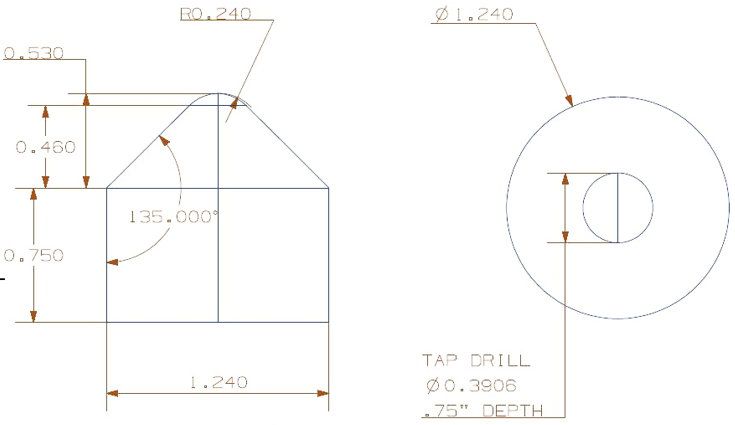
\includegraphics[width=0.7\textwidth]{design/photos/plug_gen1_drawing.PNG}
        \caption{Drawing of plug for piston valve. Measurements are in inches.}
        \label{fig:plug draw}
    \end{subfigure}
    \hfill
    \begin{subfigure}[t]{0.35\textwidth}
        \centering
        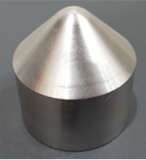
\includegraphics[width=0.58\textwidth]{design/photos/cobalt_plug.png}
        \caption{As-built plug for piston valve.}
        \label{fig:cobalt plug}
    \end{subfigure}
    %
    \caption{Drawing and picture of plug used for piston valve.}
    \label{fig:plug}
    \vspace{16pt}
\end{figure}



The plug is machined with a slope of \SI{45}{\degree} to allow for maximum flow through the valve opening. The sealing surface of the flange is machined to match this slope, and when the piston presses the plug into the flange, the plug seals into the lip machined into the flange. \Cref{fig:plug} shows the drawing for the plug, as well as a plug as-built for the piston valve. To function properly, the plug must be designed such that the force from the pressure in the driver tank a) does not overwhelm the piston opening force and b) is able to hold the plug sealed without additional pressure in the piston. Sealing with only the pressure in the driver tank allows for the the piston chambers to be empty before the valve opens, which reduces resistance for the piston's movement and therefore maximizes the piston valve opening speed. The top and bottom chamber can be seen in \Cref{fig:piston valve}, which shows the piston valve installed on its mount on the flange. The first piston valve design mount uses three (3) legs to hold the piston onto the flange, which allows for tubing to go from the connections on the flange to the connections on the piston.





% discuss design improvements in second iteration in both the mount and the o-ring
% \subsection{Design Iteration} \label{s:iteration}
% While the first plug and mount design proved the concept of a piston valve will work for the HENRI system, the seal durability was low and the piston opening was not as smooth or as fast as desired. To improve the valve, a new plug was designed using an o-ring to improve the sealing ability, and a new mount was designed to provide a more uniform and sturdy hold on the piston. The new assembly can be seen in \Cref{fig:piston assembly}. The new plug still uses a \SI{45}{\degree} slope to mate to the existing flange, but it does not go to a point like the previous design. It has a dovetail groove machined into it, as seen in \Cref{fig:Dovetail Groove}, to hold the o-ring in place such that the o-ring presses into the machined surface of the flange to strongly seal the driver tank from the test section. Two types of o-ring materials have been tested: an FFKM o-ring manufactured by Marko Rubber and a nitrile o-ring manufactured by Parker. The new mount was designed to work with the existing flange, so it uses the same bolt holes and needs to align the piston with the same sealing surface. The mount is comprised of three aluminum pieces: a circular plate mounted to the bottom of the piston, a circular plate to hold the mount on the flange, and a cylindrical support holding the two plates together and keeping the piston at the correct distance from the sealing surface. The cylindrical support has slots machined into it to allow for gas flow, tube fitting connections on the piston, and access to the bolts that mount the assembly to the flange.
